\section{Resultados}
\label{sec:resultados}

Os resultados correspondem ao cenário ambiental exploratório descrito na seção~\ref{sec:dados}. A leitura parte da rede completa para distinguir volume e concentração das atribuições e identificar as contrapartes que compõem os perfis setoriais. Em seguida, examina quais relações o filtro destaca e quanto dessa composição permanece representado no backbone.

\subsection{Contas ambientais, volume e concentração}

As duas contas totalizam 683,70 mil Gg de CO\textsubscript{2}, dos quais 392,92 mil Gg estão na diagonal de $F$ e 290,78 mil Gg nas relações entre atividades distintas em $W$. A igualdade entre os totais pela produção e pela demanda decorre da identidade contábil. A parcela intersetorial permite examinar como as mesmas emissões conectam origens e produtos finais, enquanto a diagonal situa o volume atribuído aos produtos finais da própria atividade emissora.

A rede completa tem 67 nós e 4\,290 arestas, com densidade de 97,01\%. Serviços domésticos (9700) é o único isolado: sua conta permanece na diagonal de $F$. As outras 66 atividades estão ligadas entre si nas duas direções, com graus iguais a 65. A presença de relações é compatível com a incorporação dos requisitos indiretos em $F$ e pouco distingue os perfis setoriais. O conteúdo desses perfis precisa ser examinado pela distribuição dos pesos.

Entre os 66 perfis definidos, o número efetivo varia de 1,58 a 25,04 destinos nas saídas e de 2,13 a 22,10 origens nas entradas; as medianas são 11,50 e 13,93, respectivamente. A igualdade dos graus, portanto, convive com distribuições ponderadas distintas. A Figura~\ref{fig:indicadores-resultados} permite comparar volume, concentração e seleção nas atividades de maior força intersetorial.

Três atividades permitem desenvolver esses contrastes. Energia (3500) e água, esgoto e resíduos (3680) têm as duas maiores forças de saída, com volumes próximos de 31,32 e 31,23 mil Gg, mas apresentam 20,79 e 9,88 destinos efetivos. Construção (4180), a terceira maior força de entrada, recebe 23,48 mil Gg de outras origens e tem 20,76 origens efetivas. Os casos ilustram diferenças de concentração e de direção entre atividades de grande volume intersetorial; não constituem uma amostra representativa dos perfis.

\clearpage
\begin{landscape}
\begin{figure}[p]
\centering
\caption{Volume, concentração, conectividade selecionada e cobertura em atividades de maior volume externo.}
\label{fig:indicadores-resultados}
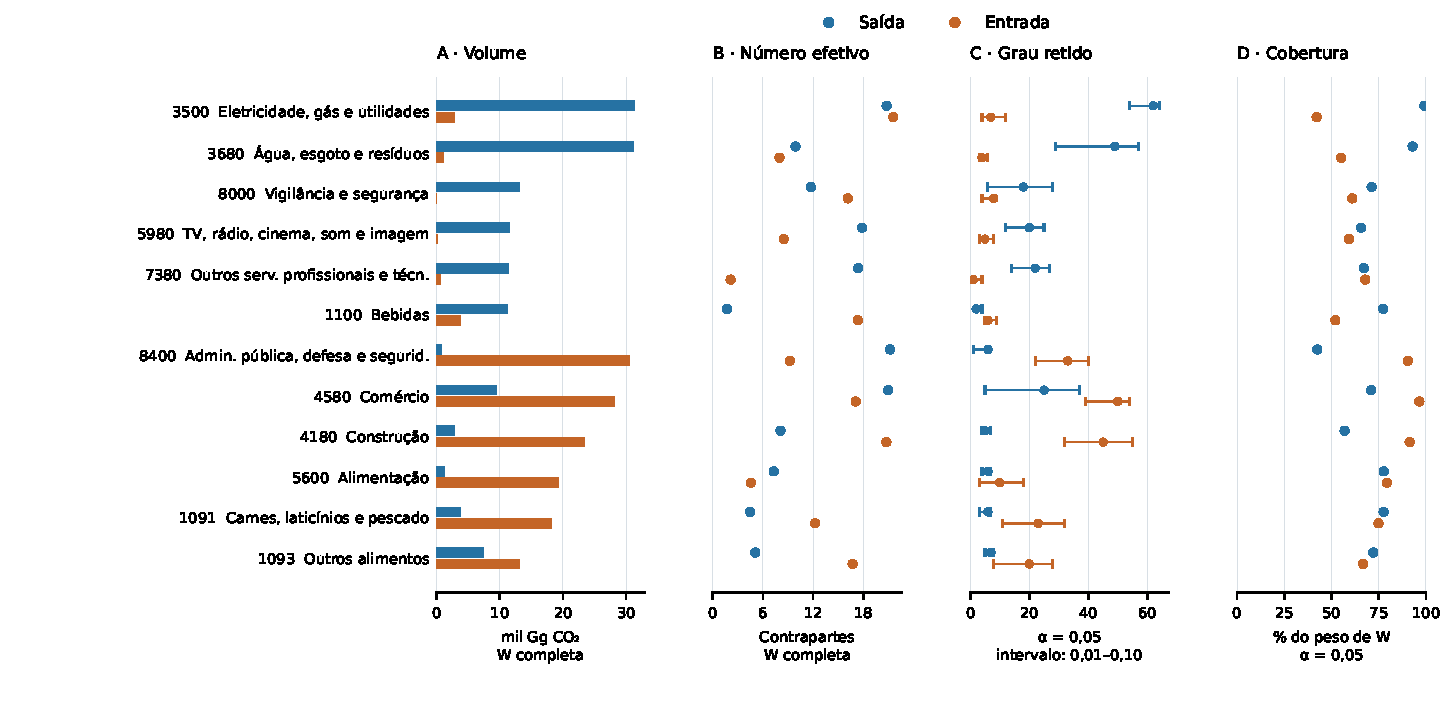
\includegraphics[width=\linewidth,height=0.80\textheight,keepaspectratio]{figuras/indicadores.pdf}
\par\smallskip
\begin{minipage}{\linewidth}\footnotesize
Fonte: elaboração própria. Linhas: união das seis maiores forças de saída e das seis maiores forças de entrada de $W$; não representam todas as atividades. Azul: saída; laranja: entrada. Volume e número efetivo são calculados em $W$ completa. Grau e cobertura referem-se a $\alpha=0{,}05$; os intervalos do grau abrangem $\alpha=0{,}01$--$0{,}10$ e não são intervalos de confiança. A diagonal é excluída.
\end{minipage}
\end{figure}
\end{landscape}

As contas completas situam esses papéis (Tabela~\ref{tab:contas-energia-construcao}). Em energia e água/resíduos, a atribuição pela produção supera a atribuição pela demanda; em construção ocorre o inverso. No entanto, construção mantém 35,91 mil Gg na diagonal, equivalentes a 92,5\% de sua conta pela produção. Sua pequena saída intersetorial corresponde a uma parcela reduzida das emissões próprias, enquanto as entradas de outras origens ampliam sua conta pela demanda. Em relação à conta pela demanda, as emissões provenientes de outras atividades correspondem a cerca de 39,5\% do total atribuído à construção; os 60,5\% restantes permanecem na diagonal.

\begin{table}[!ht]
\centering
\caption{Contas e volumes intersetoriais das atividades examinadas.}
\label{tab:contas-energia-construcao}
\small
\begin{tabular}{@{}lrrr@{}}
\toprule
Medida & Energia & Água/resíduos & Construção \\
\midrule
Produção, $c$ & 56,62 & 51,80 & 38,84 \\
Demanda, $u$ & 28,23 & 21,74 & 59,40 \\
Atribuição à própria atividade, $F_{ii}$ & 25,30 & 20,57 & 35,91 \\
Saída externa, $s^{\mathrm{out}}$ & 31,32 & 31,23 & 2,93 \\
Entrada externa, $s^{\mathrm{in}}$ & 2,92 & 1,16 & 23,48 \\
Saldo, $u-c$ & $-28,39$ & $-30,07$ & 20,56 \\
\bottomrule
\end{tabular}
\par\smallskip\begin{minipage}{\textwidth}\footnotesize
Fonte: elaboração própria. Valores em mil Gg de CO\textsubscript{2}, antes do filtro. Códigos IBGE: energia (3500), água, esgoto e gestão de resíduos (3680) e construção (4180). A diagonal integra $c$ e $u$, mas não as forças externas. Diferenças residuais entre somas de valores exibidos decorrem do arredondamento.
\end{minipage}
\end{table}





\subsection{Composição dos perfis de atribuição}
\label{sec:composicao-perfis}

A composição dos destinos ajuda a interpretar a diferença de concentração (Tabela~\ref{tab:contrapartes-completas}). O maior destino das saídas de energia é comércio, com 13,49\% do volume externo, seguido de administração pública, construção, abate e produtos de carne e agricultura. Os cinco maiores destinos reúnem 40,45\% do volume, e os demais 60 respondem por 59,55\%. A distribuição envolve produtos finais de atividades industriais, agropecuárias e de serviços.

Em água/resíduos, administração pública concentra 27,22\% das saídas externas, seguida de comércio, saúde privada, saúde pública e construção. Os cinco maiores destinos reúnem 52,35\% do volume. Assim, a maior concentração decorre, em particular, do peso da atribuição à administração pública, cuja participação é mais de três vezes a observada nas saídas de energia. Os destinos identificam atividades dos produtos finais, conforme a fronteira do modelo; não representam categorias institucionais de compradores nem apenas aquisições diretas de energia ou de serviços de água e resíduos.

Na perspectiva de entrada, construção reúne emissões de diferentes origens. Produtos de minerais não metálicos representam 12,60\% do volume externo recebido, seguidos de energia, água/resíduos, comércio e produtos de metal. As cinco maiores origens somam 38,71\%, deixando 61,29\% distribuídos entre outras 60 atividades. Sua conta pela demanda combina, portanto, as emissões atribuídas aos produtos finais da própria construção, na diagonal, com emissões intersetoriais distribuídas entre diversas origens. A posição da construção nas duas contas é esclarecida pela composição desses volumes, e não apenas pelo saldo positivo.

\begin{table}[!ht]
\centering
\caption{Principais contrapartes nos perfis completos, antes do filtro.}
\label{tab:contrapartes-completas}
\small
\begin{tabular}{@{}>{\raggedright\arraybackslash}p{0.65\textwidth}rr@{}}
\toprule
Contraparte (código IBGE) & Peso & Participação (\%) \\
\midrule
\multicolumn{3}{@{}l}{\textit{Saídas de energia (3500): produtos finais}} \\
Comércio (4580) & 4,224 & 13,49 \\
Administração pública, defesa e seguridade social (8400) & 2,556 & 8,16 \\
Construção (4180) & 2,263 & 7,23 \\
Abate e produtos de carne, laticínio e pesca (1091) & 1,930 & 6,16 \\
Agricultura (0191) & 1,693 & 5,41 \\
Demais 60 destinos & 18,650 & 59,55 \\
\midrule
\multicolumn{3}{@{}l}{\textit{Saídas de água/resíduos (3680): produtos finais}} \\
Administração pública, defesa e seguridade social (8400) & 8,501 & 27,22 \\
Comércio (4580) & 2,964 & 9,49 \\
Saúde privada (8692) & 1,672 & 5,35 \\
Saúde pública (8691) & 1,621 & 5,19 \\
Construção (4180) & 1,592 & 5,10 \\
Demais 60 destinos & 14,880 & 47,65 \\
\midrule
\multicolumn{3}{@{}l}{\textit{Entradas de construção (4180): origens emissoras}} \\
Produtos de minerais não metálicos (2300) & 2,959 & 12,60 \\
Energia elétrica, gás natural e outras utilidades (3500) & 2,263 & 9,64 \\
Água, esgoto e gestão de resíduos (3680) & 1,592 & 6,78 \\
Comércio (4580) & 1,240 & 5,28 \\
Produtos de metal, exceto máquinas e equipamentos (2500) & 1,037 & 4,42 \\
Demais 60 origens & 14,393 & 61,29 \\
\bottomrule
\end{tabular}
\par\smallskip\begin{minipage}{\textwidth}\footnotesize
Fonte: elaboração própria. Peso em mil Gg de CO\textsubscript{2}. As participações usam a força externa da atividade e direção indicadas, sem diagonal. As cinco maiores contrapartes são uma seleção de exposição, sem alterar $W$ ou aplicar corte adicional. Nomes abreviados; valores calculados sem arredondamento no notebook. A relação energia $\rightarrow$ construção aparece nas duas perspectivas e não deve ser somada duas vezes em totais da rede.
\end{minipage}
\end{table}

As direções inversas também distinguem os dois casos. Energia recebe 2,92 mil Gg de outras origens, com 21,59 origens efetivas; construção distribui 2,93 mil Gg a outros produtos finais, com 8,10 destinos efetivos. Neste último perfil, administração pública reúne 31,21\% do volume externo. Mesmo com forças próximas, a distribuição das saídas de construção é mais concentrada do que a das entradas de energia. Cada nó precisa, assim, ser interpretado nos dois papéis que exerce na rede.

A composição dos perfis esclarece a passagem entre as contas. Em energia e água/resíduos, as saídas para outros produtos finais superam as entradas de outras origens, reduzindo a atribuição pela demanda em relação à produção. Em construção, as entradas superam as saídas e elevam essa atribuição. A diagonal integra as duas contas e cancela na diferença; as contrapartes identificadas mostram quais relações intersetoriais compõem os saldos.

\clearpage
\subsection{Seleção das relações e limites de cobertura}

O backbone de referência preserva 575 arestas, ou 13,40\% das ligações de $W$, e 70,69\% do peso intersetorial (Tabela~\ref{tab:sensibilidade-backbone}). Na Figura~\ref{fig:matriz-backbone}, a linha de energia e a coluna de construção mostram a extensão das relações retidas nesses dois perfis. O painel de pesos diferencia os volumes dessas ligações: a seleção por importância local não implica pesos absolutos semelhantes.

\begin{table}[htbp]
\centering
\caption{Sensibilidade da seleção e da cobertura ao parâmetro do filtro.}
\label{tab:sensibilidade-backbone}
\small
\begin{tabular}{@{}crrrr@{}}
\toprule
$\alpha$ & Arestas & \% das arestas de $W$ & Peso retido & Cobertura (\%) \\
\midrule
0,01 & 338 & 7,88 & 166,88 & 57,39 \\
0,05 & 575 & 13,40 & 205,55 & 70,69 \\
0,10 & 755 & 17,60 & 224,92 & 77,35 \\
\bottomrule
\end{tabular}
\par\smallskip\begin{minipage}{\textwidth}\footnotesize
Fonte: elaboração própria. Peso em mil Gg de CO\textsubscript{2}. Cobertura relativa ao peso de $W$, sem diagonal. Todos os casos mantêm 67 nós, um isolado e um componente fracamente conectado de 66 atividades. O filtro é aplicado à mesma rede completa, com regra OU e sem atualização dos perfis.
\end{minipage}
\end{table}

A cobertura agregada oculta perdas locais. Em $\alpha=0{,}05$, as menores coberturas são 32,96\% nas saídas e 33,79\% nas entradas. Portanto, preservar parcela expressiva do peso total não assegura representação igualmente completa de cada atividade e direção.

A mudança de $\alpha$ altera as posições individuais por grau, embora o componente de 66 atividades permaneça nos três casos. A conectividade agregada não demonstra estabilidade das posições setoriais. Os valores detalhados das mudanças, a decomposição da seleção por extremidade e a sensibilidade dos perfis focais constam do \ref{anexo:diagnosticos}; $0{,}05$ permanece como referência, sem ser considerado um parâmetro ótimo.





\clearpage
\begin{landscape}
\begin{figure}[p]
\centering
\caption{Matriz de adjacência do backbone com $\alpha=0{,}05$: (a) presença das arestas.}
\label{fig:matriz-backbone}
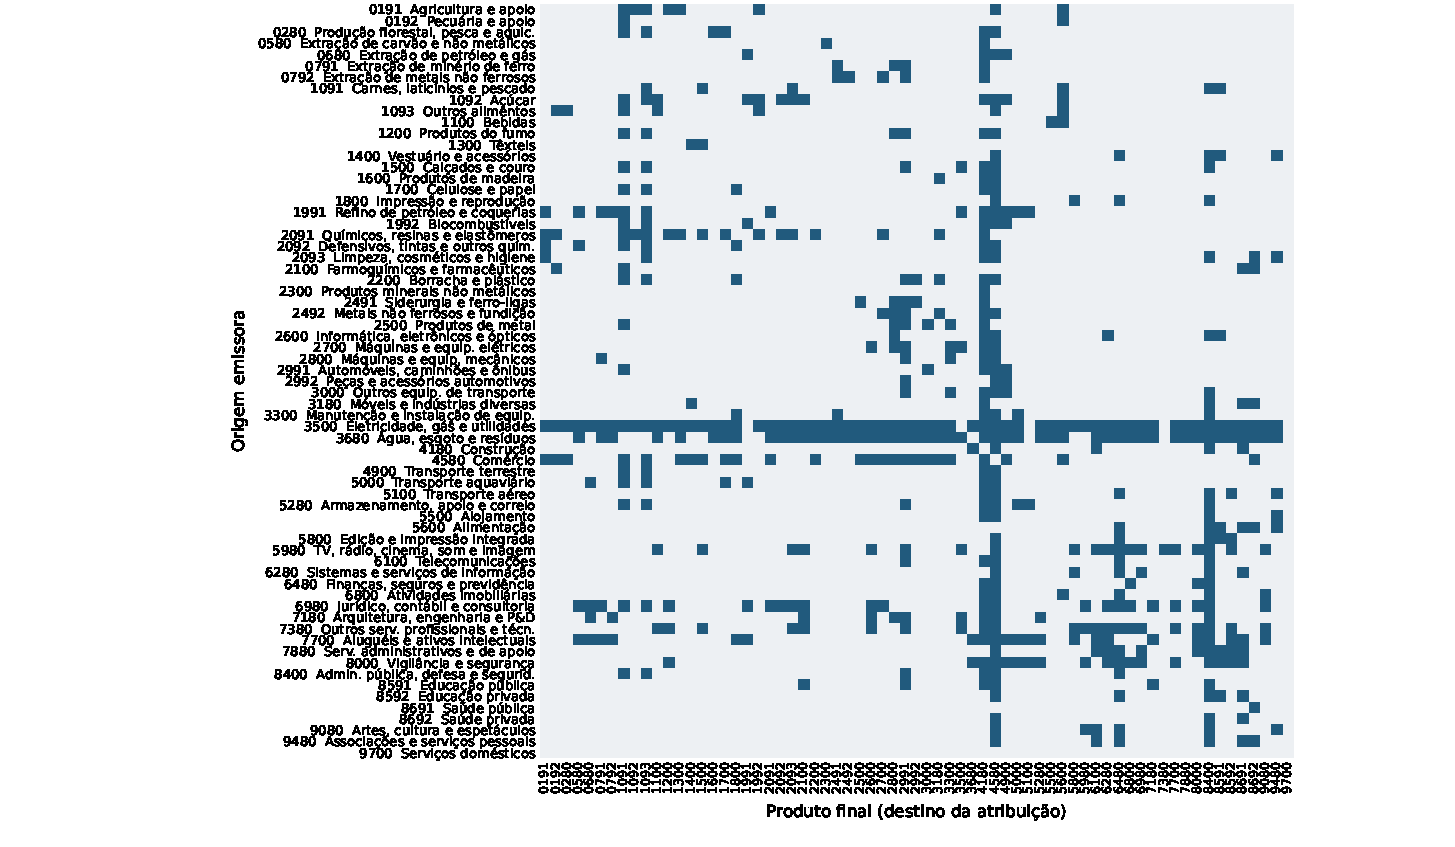
\includegraphics[width=\linewidth,height=0.82\textheight,keepaspectratio]{figuras/matriz_presenca.pdf}
\par\smallskip
\begin{minipage}{\linewidth}\footnotesize
Fonte: elaboração própria. Linha: origem emissora; coluna: atividade do produto final. Ordem setorial do IBGE nos dois eixos. Azul identifica as 575 ligações retidas; cinza indica ausência no backbone, inclusive a diagonal. Ausência no backbone não implica valor nulo em $F$ ou $W$. Todas as 67 atividades permanecem nos eixos.
\end{minipage}
\end{figure}
\clearpage
\begin{figure}[p]
\ContinuedFloat
\centering
\caption{Matriz de adjacência do backbone com $\alpha=0{,}05$: (b) pesos das mesmas arestas.}
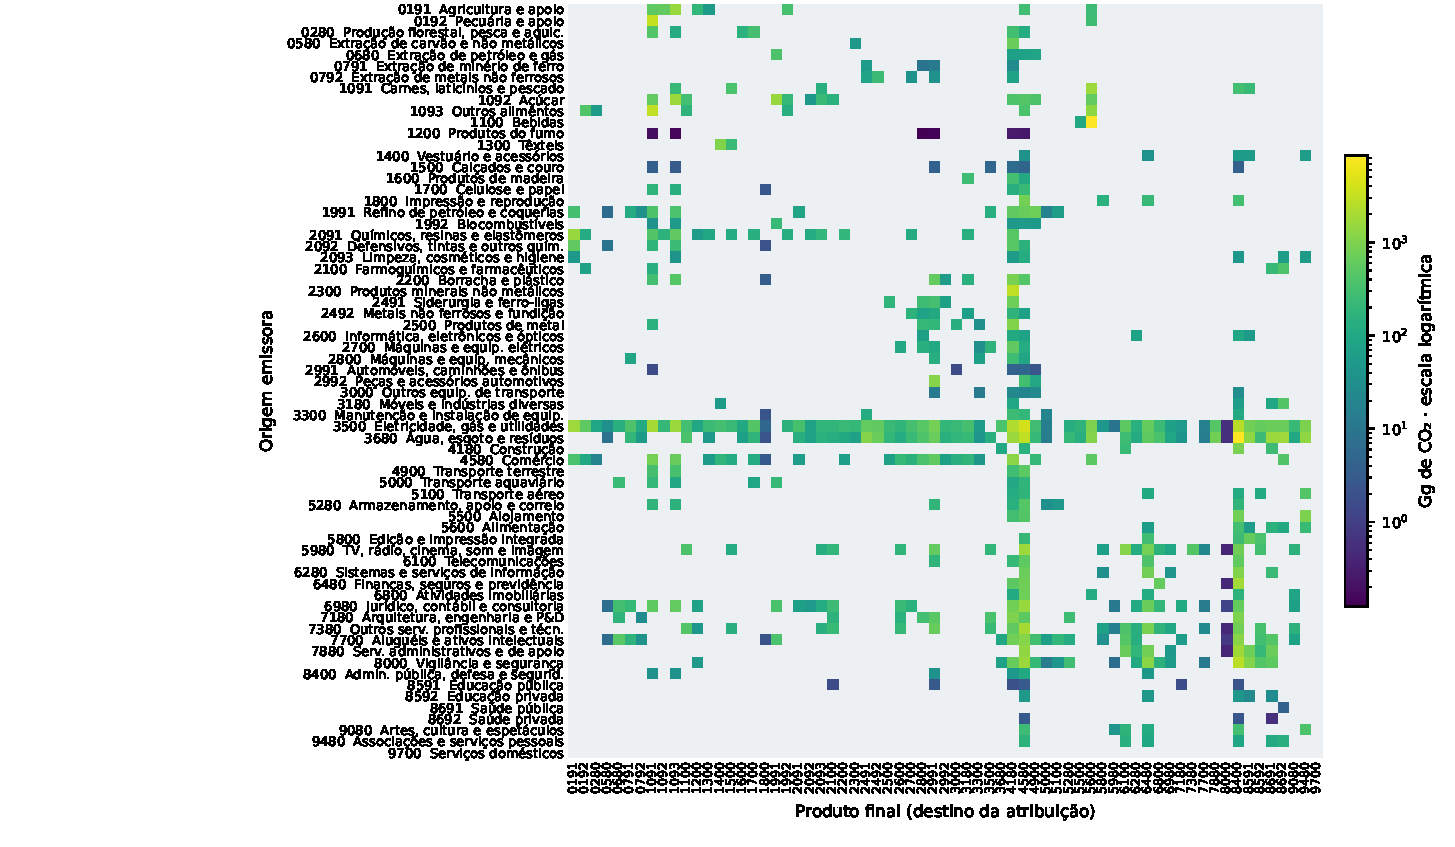
\includegraphics[width=\linewidth,height=0.82\textheight,keepaspectratio]{figuras/matriz_peso.pdf}
\par\smallskip
\begin{minipage}{\linewidth}\footnotesize
Fonte: elaboração própria. Mesma ordem e mesma seleção do painel (a). A cor representa pesos originais em Gg de CO\textsubscript{2}, em escala logarítmica, sem normalização por linha ou coluna. Cinza identifica células sem aresta retida. A cor mede volume absoluto; a concentração é descrita pelos números efetivos em $W$ completa.
\end{minipage}
\end{figure}
\end{landscape}

\subsection{Importância local nas duas perspectivas da relação}

Os perfis completos mostram como os pesos se distribuem; o filtro acrescenta a avaliação da importância local de cada relação para suas duas extremidades. As cores da Figura~\ref{fig:rede-focos} evidenciam o predomínio de saídas no recorte de energia e de entradas no de construção, mantendo as demais relações do mesmo backbone ao fundo. O motivo da retenção e a cobertura, apresentados na Tabela~\ref{tab:motivos-casos} e nos painéis do \ref{anexo:paineis}, permitem interpretar essa diferença entre as duas vistas.

\begin{table}[htbp]
\centering
\caption{Motivos de retenção e cobertura nos recortes de energia e construção.}
\label{tab:motivos-casos}
\small
\begin{tabular}{@{}lrrrrr@{}}
\toprule
Recorte & Arestas & Só saída & Só entrada & Ambos & Cobertura (\%) \\
\midrule
Energia: entradas & 7 & 1 & 5 & 1 & 42,1 \\
Energia: saídas & 62 & 0 & 56 & 6 & 99,2 \\
Construção: entradas & 45 & 41 & 0 & 4 & 91,4 \\
Construção: saídas & 5 & 4 & 1 & 0 & 57,0 \\
\bottomrule
\end{tabular}
\par\smallskip\begin{minipage}{\textwidth}\footnotesize
Fonte: elaboração própria. $\alpha=0{,}05$. Saída e entrada nas colunas de motivo identificam o teste na origem e no destino da aresta, independentemente da atividade em destaque. Cobertura: peso retido dividido pela força da mesma atividade e direção em $W$. Os recortes compartilham arestas e não devem ser somados para obter totais da rede.
\end{minipage}
\end{table}

Em energia, 56 das 62 saídas retidas passam somente pelo teste de entrada no destino. Energia tem participação destacada na composição externa de muitas demandas finais, embora cada destino possa representar parcela pequena das emissões distribuídas pela origem. Por exemplo, energia $\rightarrow$ alimentação (5600) representa 3,00\% das saídas externas de energia e 4,86\% das entradas externas de alimentação. A relação é selecionada somente na perspectiva do destino, evidenciando a diferença entre a composição recebida por uma atividade e a distribuição das emissões pela outra.

Em construção, 41 das 45 entradas passam somente pelo teste de saída na origem. Construção representa parcela destacada das atribuições externas dessas origens, mesmo quando a contribuição individual é pequena no total recebido pelo destino. Produtos de metal (2500) $\rightarrow$ construção, por exemplo, corresponde a 32,57\% das saídas externas da origem e a 4,42\% das entradas externas do destino. O filtro retém essa ligação somente pelo teste de saída na origem. Ela identifica uma demanda final que concentra parte expressiva das atribuições externas de produtos de metal, mesmo ocupando uma posição menor na composição recebida por construção.

As entradas de construção selecionadas pelos dois testes vêm de produtos de minerais não metálicos, energia, água/resíduos e comércio. A relação energia $\rightarrow$ construção, comum aos dois recortes, pesa aproximadamente 2\,263 Gg: 7,23\% das saídas externas de energia e 9,64\% das entradas externas de construção. Sua seleção nas duas extremidades conecta os papéis predominantes dos dois casos.

As saídas de energia e as entradas de construção têm as maiores coberturas dos respectivos recortes (Tabela~\ref{tab:motivos-casos}). Nas direções inversas, as listas curtas não autorizam desprezar as relações omitidas em conjunto. Tampouco a diferença entre 62 saídas de energia e 45 entradas de construção indica concentração distinta: na rede completa, os respectivos números efetivos são próximos, ambos de 20,8 contrapartes.

A sensibilidade qualifica a leitura desses papéis. Entre $\alpha=0{,}01$ e $0{,}10$, energia mantém de 54 a 64 saídas, com cobertura de 92,12\% a 99,96\%, enquanto construção mantém de 32 a 55 entradas, com cobertura de 74,31\% a 97,76\% (Tabela~\ref{tab:sensibilidade-casos}). Em todos os parâmetros, predomina o teste somente de entrada no destino nas saídas de energia e somente de saída na origem nas entradas de construção. Os cinco maiores destinos de energia permanecem selecionados. Esses resultados sustentam a leitura dos papéis ilustrados dentro da faixa examinada, apesar das mudanças no número de ligações e na cobertura.

A permanência de cada relação, contudo, exige verificação própria. Entre as cinco maiores origens de construção, água/resíduos deixa de ser selecionada em $\alpha=0{,}01$, embora represente 6,78\% do perfil externo recebido. Energia $\rightarrow$ construção permanece selecionada pelos dois testes nos três parâmetros. A composição da rede completa e os saldos não mudam com $\alpha$; a instabilidade de uma ligação no backbone delimita sua seleção sob o modelo nulo, sem alterar o volume de sua atribuição.



\clearpage
\begin{figure}[p]
\centering
\caption{Duas perspectivas do mesmo backbone: (a) destaque para energia (3500).}
\label{fig:rede-focos}
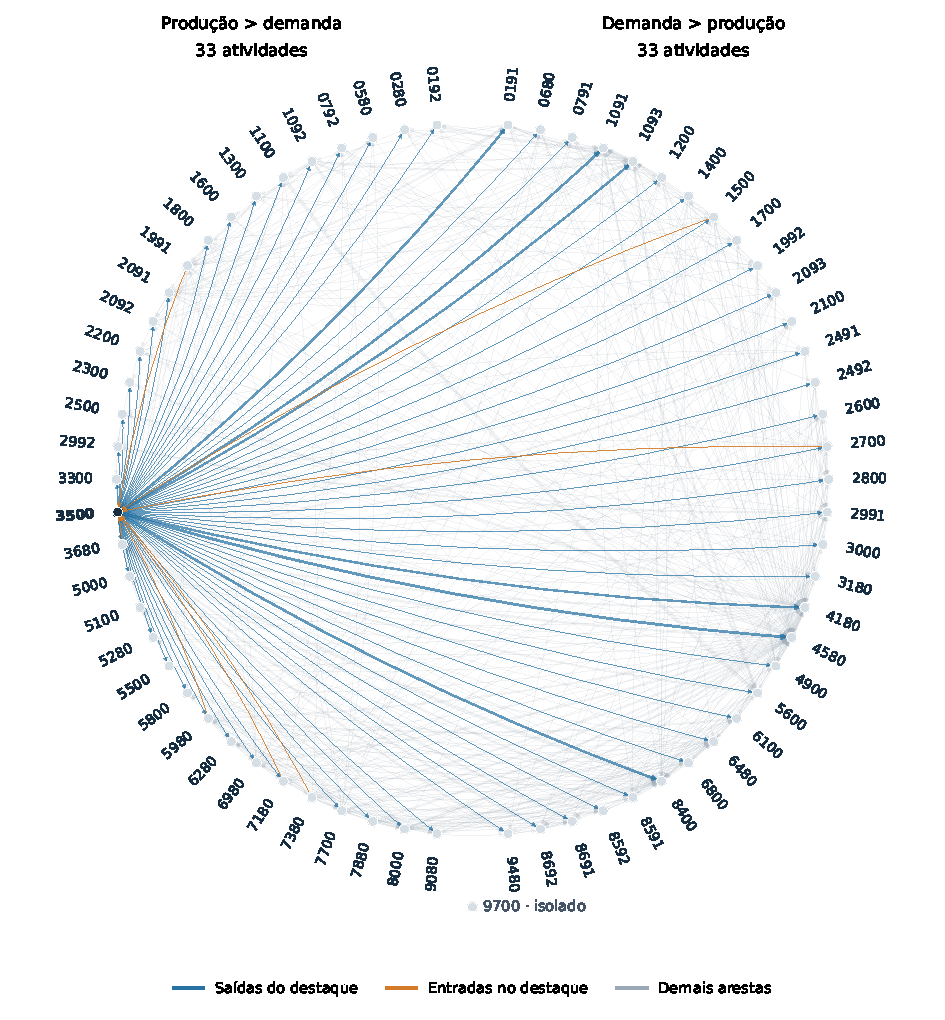
\includegraphics[width=\textwidth,height=0.76\textheight,keepaspectratio]{figuras/rede_foco_3500.pdf}
\par\smallskip
\begin{minipage}{\textwidth}\footnotesize
Fonte: elaboração própria. Cada vista mantém 67 nós e 575 arestas em $\alpha=0{,}05$. Azul: saídas do destaque; laranja: entradas; cinza: demais arestas. Energia tem 62 saídas e sete entradas, com cobertura de 99,2\% e 42,1\% do volume externo de cada direção. Área dos nós uniforme; espessura cresce com a raiz quadrada do peso. Posição definida pelo sinal de $u-c$ e pela ordem IBGE: 33 nós com $c>u$ à esquerda, 33 com $u>c$ à direita e o isolado abaixo. A disposição não resulta de centralidade ou comunidade.
\end{minipage}
\end{figure}
\clearpage
\begin{figure}[p]
\ContinuedFloat
\centering
\caption{Duas perspectivas do mesmo backbone: (b) destaque para construção (4180).}
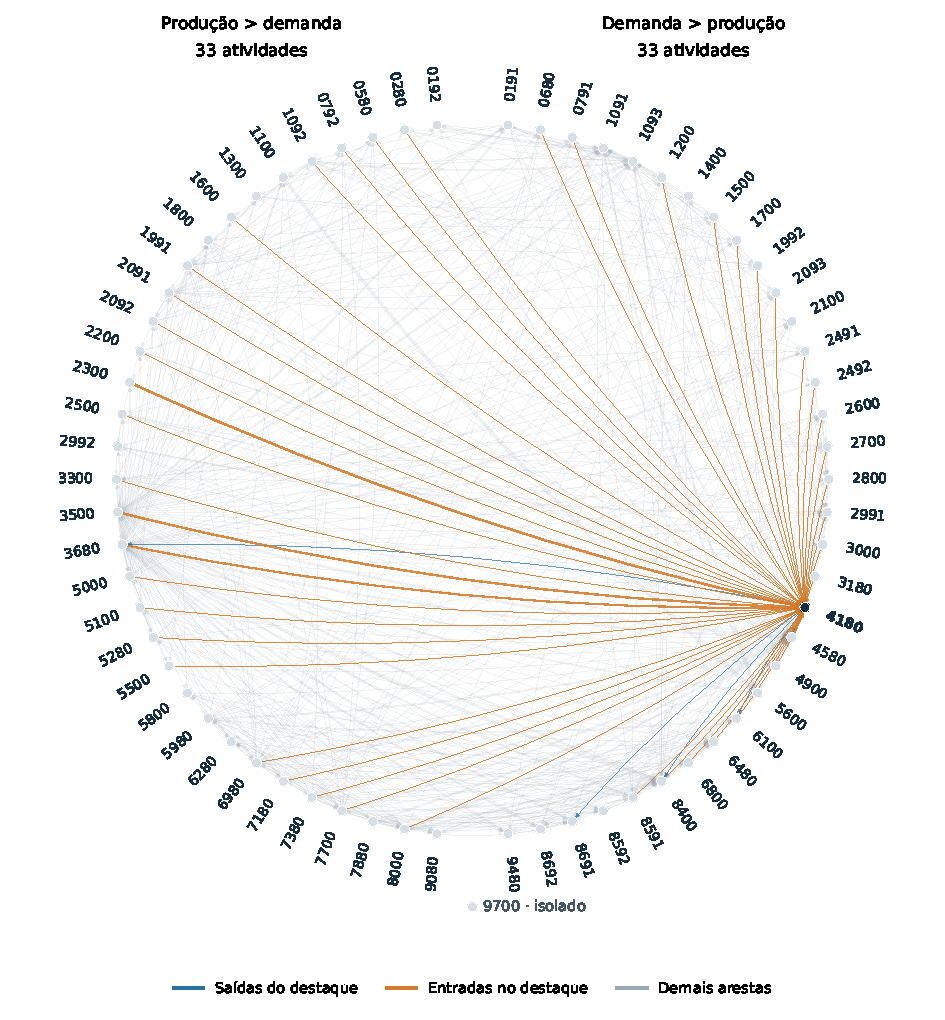
\includegraphics[width=\textwidth,height=0.76\textheight,keepaspectratio]{figuras/rede_foco_4180.pdf}
\par\smallskip
\begin{minipage}{\textwidth}\footnotesize
Fonte: elaboração própria. Mesmos nós, arestas, posições e escala de espessura do painel (a). Construção tem cinco saídas e 45 entradas, com cobertura de 57,0\% e 91,4\%. Cores representam direção em relação ao destaque, não motivo de retenção. As duas vistas preservam 70,69\% do peso intersetorial de $W$. Cruzamentos e proximidade não representam trajetórias ou distâncias econômicas; relações individuais podem ser consultadas na matriz e nos painéis do anexo.
\end{minipage}
\end{figure}
\clearpage
